\documentclass{article}


\usepackage{fancyhdr}
\usepackage{extramarks}
\usepackage{amsmath}
\usepackage{amsthm}
\usepackage{amsfonts}
\usepackage{tikz}
\usepackage[plain]{algorithm}
\usepackage{algpseudocode}
\usepackage{enumerate}
\usepackage{tikz}
\usepackage{listings}
\usepackage{hyperref}
\usepackage{subfigure}
\usepackage[graphicx]{realboxes}
\usepackage{xcolor}
\usepackage{color}



% 代码块高级设置
\lstset{
% basicstyle=\footnotesize,                 % 设置整体的字体大小
showstringspaces=false,                     % 不显示字符串中的空格
frame=single,                               % 设置代码块边框
numbers=left,                               % 在左侧显示行号
% numberstyle=\footnotesize\color{gray},    % 设置行号格式
numberstyle=\color{darkgray},               % 设置行号格式
backgroundcolor=\color{white},              % 设置背景颜色
keywordstyle=\color{blue},                  % 设置关键字颜色
commentstyle=\it\color[RGB]{0,100,0},       % 设置代码注释的格式
stringstyle=\sl\color{red},                 % 设置字符串格式
}

\hypersetup{hidelinks,
	colorlinks=true,
	allcolors=black,
	pdfstartview=Fit,
	breaklinks=true}

%
% Basic Document Settings
%  

\topmargin=-0.45in
\evensidemargin=0in
\oddsidemargin=0in
\textwidth=6.5in
\textheight=9.0in
\headsep=0.25in

\linespread{1.1}

\pagestyle{fancy}
\lhead{}
\chead{\hmwkClass : \hmwkTitle}
\rhead{\firstxmark}
\lfoot{\lastxmark}
\cfoot{\thepage}

\renewcommand\headrulewidth{0.4pt}
\renewcommand\footrulewidth{0.4pt}

\setlength\parindent{0pt}



%
% Homework Details
%   - Title
%   - Due date
%   - Class
%   - Instructor
%   - Class number
%   - Name
%   - Student ID

\newcommand{\hmwkTitle}{Problem Set 1 Document}
\newcommand{\hmwkDueDate}{October 18th}
\newcommand{\hmwkClass}{Parallel Computing}
\newcommand{\hmwkClassInstructor}{Professor Rui Fan}

% 正式选课名单确定之后,根据通知填写所在班级编号

\newcommand{\hmwkAuthorName}{Zhenghong Yu}
\newcommand{\hmwkAuthorMail}{yuzhh1@shanghaitech.edu.cn}
\newcommand{\hmwkAuthorID}{2020533156}


%
% Title Page
%

\title{
    \vspace{2in}
    \textmd{\textbf{\hmwkClass:\\  \hmwkTitle}}\\
    \normalsize\vspace{0.1in}\small{Due\ on\ \hmwkDueDate\ at 23:59 }\\
   \vspace{2in}
}

\author{
    Mailbox: \hmwkAuthorMail\\
	Student ID: \hmwkAuthorID\\
    Student Name: \hmwkAuthorName}
\date{}




\begin{document}

\maketitle
\pagebreak
\tableofcontents

\pagebreak





\section{Problem 1}
\subsection{Question 1}
\textcolor[rgb]{0,0,1}{\textbf{Consider the problem of adding a list of $n$ numbers. Assume that one person can add two numbers in time $t_{c}$. How long will one person take to add $n$ numbers?}}\\
\textbf{Solution: } (n-1)$t_{c}$
\subsection{Question 2}
\textcolor[rgb]{0,0,1}{\textbf{Now assume eight people are available for adding these $n$ numbers and that the list has already been divided into eight equal parts. Each person can add two numbers in time $t_{c}$. Furthermore, a person can pass on the result of an addition (in the form of a single number) to the person sitting next to him or her in time $t_{w}$. How long will it take to add $n$ numbers if\\\\
a) All eight people sat in a circle.\\ 
b) The eight people are sitting in two rows of four people each.\\}}
\textbf{Solution: }\\
a) $(\frac{n}{8}+2)t_{c}+4t_{w}$ \\
b) $(\frac{n}{8}+2)t_{c}+3t_{w}$ 
\subsection{Question 3}
\textcolor[rgb]{0,0,1}{\textbf{If you are free to seat the eight people in any configuration, how would you seat them as to minimize the time taken to add the list of numbers? Is there a best configuration independent of $t_{c}$ and $t_{w}$?}}\\
\textbf{Solution: }\\
I'll let the eight people sit in a cube, which will take $(\frac{n}{8}+2)t_{c}+3t_{w}$. There is not a best configuration independent of $t_{c}$ and $t_{w}$.
\section{Problem 2}
\textcolor[rgb]{0,0,1}{\textbf{Compare the execution of the following code to calculate the greatest common divisor of $x$ and $y$ as performed on a SIMD versus an MIMD architecture. }}
\begin{lstlisting}[language=c++]
gcd (x,y) {
while (x != y) {
    if (x > y) x = x-y;
    else y = y-x;
    }
}
\end{lstlisting}
\textcolor[rgb]{0,0,1}{\textbf{Suppose two arrays $x = (x_{0},\cdots, x_{n-1})$ and $y = (y_{0},\cdots, y_{n-1})$ are each distributed across $n$ processors with $x_{i}$ and $y_{i}$ on processor $i$. We wish to find $z = (z_{0},\cdots, z_{n-1})$, where $z_{i} = gcd(x_{i}, y_{i})$. Assuming that a compare or a subtract instruction 
each takes one time step, how many time steps would it take to calculate the 
result when $x = (52,24)$ and $y = (12, 64)$ using\\
a) A two processor SIMD architecture. \\ 
b) A two processor MIMD architecture. \\
In each case, write a trace for the two processors, indicating clearly which 
instruction is executed at which time step.\\}}
\textbf{Solution: }\\
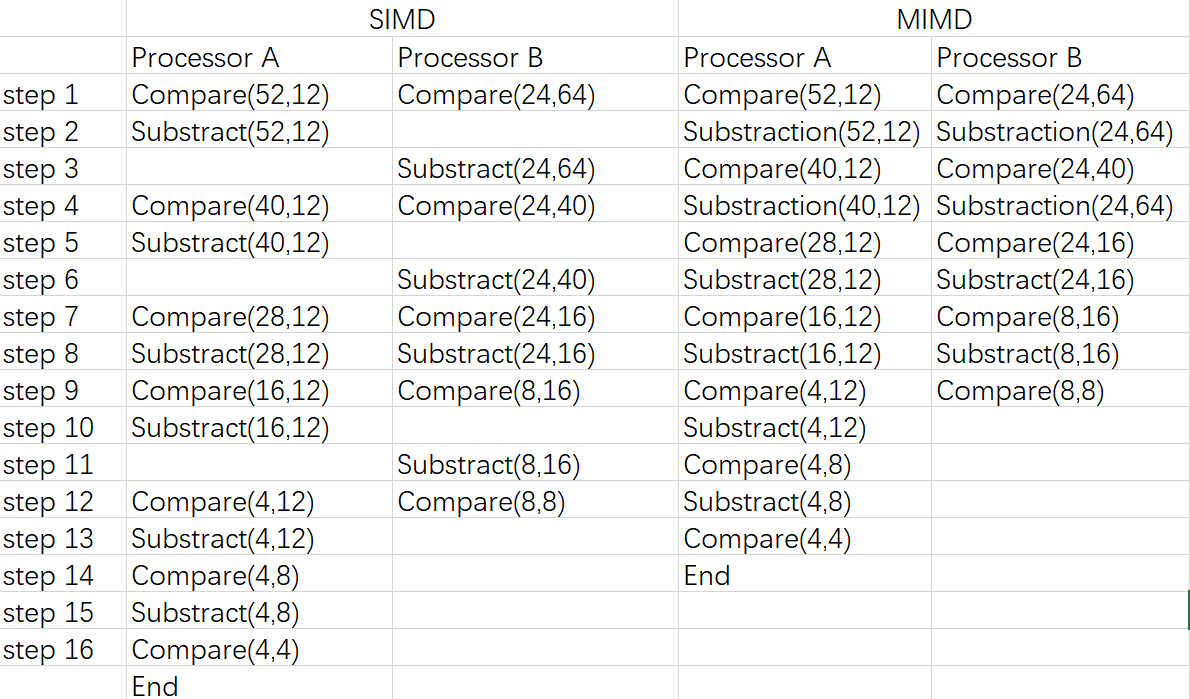
\includegraphics[scale=0.4]{list1.png}

\section{Problem 3}
\textcolor[rgb]{0,0,1}{\textbf{A $perfect\ shuffle$ for a set of $2^n$ processors consists of connecting each processor $i$ to another processor $j$ whose ID in binary is a left rotation of $i$'s ID in binary. A perfect shuffle on 8 processors is shown below. For example, the left rotation of 100 is 001 (the 1 bit wraps around to the right side), so there is an edge between 100 and 001.\\\\
A switch consists of two inputs $x$ and $y$ and two outputs. If the inputs are passed 
through the switch, then the outputs are also $x$ and $y$. Otherwise, the inputs are 
crossed, and the outputs are $y$ and $x$. A switch is shown below.\\\\
}}
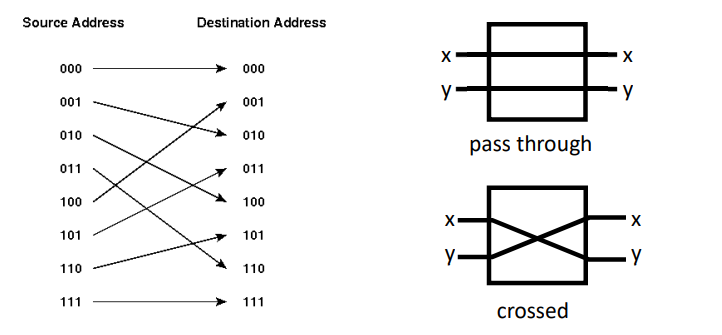
\includegraphics[scale=0.5]{fig1.png}\\\\
\textcolor[rgb]{0,0,1}{\textbf{An $Omega\ network$ for a set of $2^n$ processors is an indirect network consisting of $n$ layers of perfect shuffles of the processors. Switches in the network can be set to either pass through or crossed in order to perform routing. For example, in the Omega network below, switches 1B, 2C and 3A are set to pass through to route from processor 001 to 001, while switch 2D is set to pass through and switches 1D and 3D are set to crossed to route from 011 to 110. }}
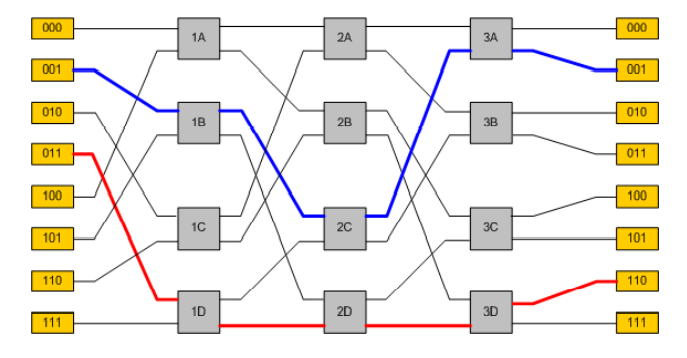
\includegraphics[scale=0.6]{fig2.png}\\
\textcolor[rgb]{0,0,1}{\textbf{For this problem, devise an algorithm to route a message between two 
processors in an Omega network. Explain why your algorithm is correct. \\}}
\textbf{Solution: }\\
For each pair of processors:
\begin{itemize}
	\item First determine the digits of the source processor which differ to to the destination processor.
	\item Then, for the $i$th layer of Omega network, set the switch as pass cross if the $i$ digit of the source processor is differ to the destination processor, otherwise set it as pass though.
\end{itemize}
We can know that each layer help to change the corresponding bit of processor ID, the algorithm is like a XOR gate to find the correct destination.

\section{Problem 4}
\textcolor[rgb]{0,0,1}{\textbf{The task graph shown in the figure below represents a parallel application. Each circle represents an indivisible task. There are 12 tasks: an initialization task, 10 
computation tasks, and a finalization task. Each of the 12 tasks takes exactly one unit of time on one processor. The initialization task must complete before any of the computation tasks begin. Similarly, all 10 computation tasks must complete before the finalization task begins. The computation tasks can be 
executed in any order.\\}}
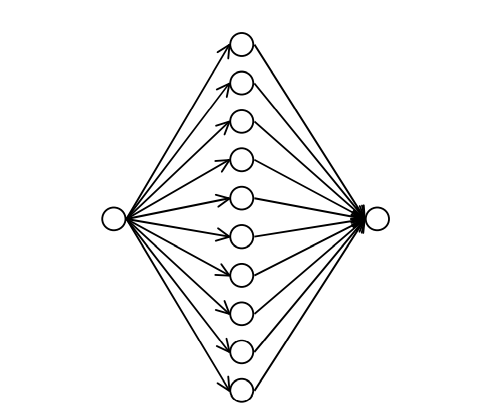
\includegraphics[scale=0.6]{fig3.png}\\
\subsection{Question 1}
\textcolor[rgb]{0,0,1}{\textbf{What is the maximum speedup that can be achieved if this problem is 
solved on a parallel computer with 2 processors? Give a diagram showing how the tasks would be allocated to processors.}}\\
\textbf{Solution: }\\
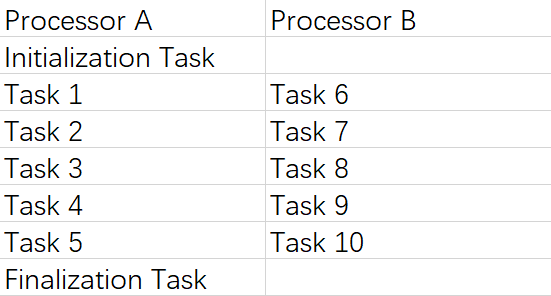
\includegraphics[scale=0.5]{list2.png}\\
The time speedup is $\frac{12}{7}$
\subsection{Question 2}
\textcolor[rgb]{0,0,1}{\textbf{b) What is the maximum speedup that can be achieved if this problem is 
solved on any parallel computer?}}\\
Based on Amdahl's law, the maximum speedup is:
$$S_{p} = \frac{12}{2+\frac{10}{p}}$$
Since the minimum value of $\frac{10}{p} = 1$ as one single task must finished by one processor, we can get
$$max\{S_{p}\} = \frac{12}{2+1} = 4$$
\subsection{Question 3}
\textcolor[rgb]{0,0,1}{\textbf{What is the minimum number of processors required to achieve the 
speedup given in part (b)? Give a diagram showing how the tasks would 
be allocated to processors. }}\\
\textbf{Solution: }\\
We need at least 10 processors to achieve the speedup given in part(b)\\
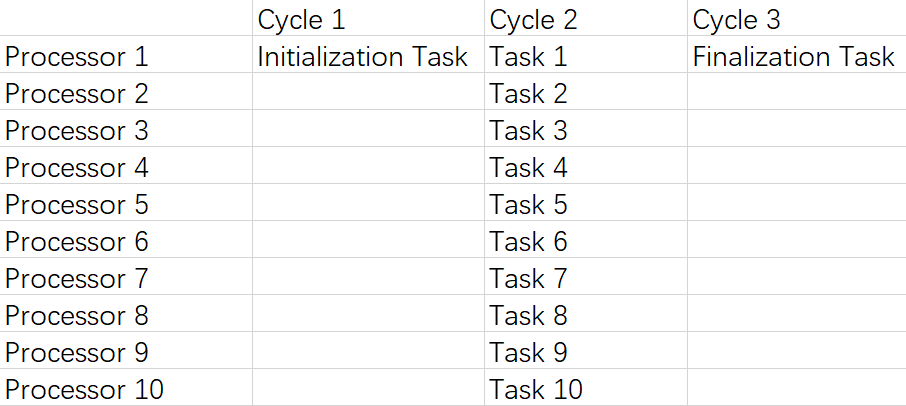
\includegraphics[scale=0.5]{list3.png}
\section{Problem 5}
\textcolor[rgb]{0,0,1}{\textbf{Three students taking the Parallel Computing course have written parallel 
programs for their lab assignments. }}\\
\subsection{Question 1}
\textcolor[rgb]{0,0,1}{\textbf{Amanda's parallel program achieves a speedup of 9 on 10 processors. What is the maximum fraction $f$ of the computation that can be inherently sequential in her program? }}\\
\textbf{Solution: }\\
Based on Amdahl's law, we have
$$S_{p} = \frac{1}{f+(1-f)/p}$$
where $p=10$, $S_{p}=9$, we can get $f=\frac{1}{81}$. So the maximum fraction $f$ of the computation that can be inherently sequential in her program is $\frac{1}{81}$.
\subsection{Question 2}
\textcolor[rgb]{0,0,1}{\textbf{Brian's parallel program executes in 225 seconds on 16 processors. By 
timing parts of his program, he determines that 9 seconds is spent performing initialization and finalization on one processor, and for the remaining 216 seconds all 16 processors are executing. What is the $scaled\ speedup$ achieved by Brian's program?}}\\
\textbf{Solution: }\\
$$S_{p}=\frac{fT_{1}+p(1-f)T_{1}}{T_{1}}=15.4$$
\subsection{Question 3}\
\textcolor[rgb]{0,0,1}{\textbf{Cindy times her parallel program on 10 processors and finds that for 270 
seconds, all processors are active, and for 30 seconds, one processor is executing inherently sequential code. Assuming that the size of the sequential code does not increase as the problem size increases, what is the scaled speedup she can expect for p processors, where p = 20, 30, 40? }}\\
\textbf{Solution: }\\
$$S_{p}=\frac{30+270\cdot p}{30+270}=\frac{1+9p}{10}$$
Thus $S_{p}(20)=18.1$, $S_{p}(30)=27.1$, $S_{9}(40)=36.1$.


\section{Problem 6}
\subsection{Question 1}
\textcolor[rgb]{0,0,1}{\textbf{Suppose we have a problem for which there is a sequential algorithm running in time $n$ on an input of size $n$. Now, consider a parallel algorithm for the problem which has parallel running time $n/p + 2log p$ when using $p$ processors. Is it possible to maintain isoefficiency for this parallel algorithm? If so, give the necessary relationship between $n$ and $p$. }}\\
\textbf{Solution: }\\
$$E=\frac{n}{p*(\frac{n}{p}+2\log p)}=\frac{1}{1+\frac{2p\log p}{n}}$$
To maintian the isoefficiency, $n\in \Omega (p\log p)$

\subsection{Question 2}
\textcolor[rgb]{0,0,1}{\textbf{Suppose now the sequential running time is $n^2$ and the parallel running time is $n^2/p + n^3/\sqrt{p}$. Can this algorithm algorithm maintain 
isoefficiency, and if so, what is the necessary relationship between $n$ and $p$?}}\\
\textbf{Solution: }\\
$$E=\frac{n^2}{p*(\frac{n^2}{p}+\frac{n^3}{\sqrt{p}})}=\frac{1}{1+n\sqrt{p}}$$
To maintain the isoefficiency, $n\Theta (\frac{1}{\sqrt{p}})$














\end{document}
